\documentclass[a4paper,12pt]{article}
\usepackage[utf8]{inputenc}
\usepackage{graphicx}
\usepackage{hyperref}
\usepackage{amsmath}
\usepackage{fancyhdr}

% Page formatting
\pagestyle{fancy}
\fancyhf{}
\fancyhead[L]{Software Tools And Technology}
\fancyfoot[C]{\thepage}

\begin{document}

% Title Page
\begin{center}
    \Large \textbf{Software Tools And Technology} \\[1cm]
\begin{figure}[h!]
   \centering
    
\includegraphics[width=0.3\linewidth]{makaut logo.png}
\end{figure}
\vspace{0.5 cm}
    
    Group 2: \\[1cm]
    \textbf{Lab Notebook} \\[2cm]

    \vspace{0.1 cm}

    
    \textbf{Group members:} \\[0.5cm]
    1. Rajkumar Pal - Leader (BCA) \\[0.2cm]
    2. Jahir Mondal BSc IT(AI) \\[0.2cm]
    3. Arnab Pandit BSc IT(CS) \\[0.2cm]
    4. Pritam Pratihar (BCA) \\[0.2cm]
    5. Suhana Pervaze (BCA) \\[2cm]

    \textbf{Instructor}: Dr. Ayan Ghosh \\[0.5cm]
    Course: Software Tools And Technology
\end{center}

% Lab Notebook Entries
\section*{Lab Notebook Entries Index}

\subsection*{1. Lab Entry by Rajkumar Pal}
\subsubsection*{1.1 Experiment}
\begin{tabbing}
    Sl. No. \hspace{2cm} \= Assignments \\
    1. \> Introduction to Github and Github desktop version installation \\
\end{tabbing}

\subsection*{2. Lab Entry by Jahir Mondal}
\subsubsection*{2.1 Experiment}
\begin{tabbing}
    Sl. No. \hspace{2cm} \= Assignments \\
    1. \> Converting Submit button to Chin Tapak Dum Dum \\
\end{tabbing}

\subsection*{3. Lab Entry by Arnab Pandit}
\subsubsection*{3.1 Experiment}
\begin{tabbing}
    Sl. No. \hspace{2cm} \= Assignments \\
    1. \> Making calculator in C \\
\end{tabbing}

\subsection*{3. Lab Entry by Pritam Pratihar}
\subsubsection*{3.1 Experiment}
\begin{tabbing}
    Sl. No. \hspace{2cm} \= Assignments \\
    1. \> Creating LaTeX Repository in GitHub \\
\end{tabbing}

\subsection*{3. Lab Entry by Suhana Pervaze}
\subsubsection*{3.1 Experiment}
\begin{tabbing}
    Sl. No. \hspace{2cm} \= Assignments \\
    1. \> Introduction to LaTeX \\
\end{tabbing}

\newpage

% Entry 1: Rajkumar Pal
\section*{Lab Entry By Rajkumar Pal}

\subsection*{1. Introduction to GitHub and GitHub Desktop Version Installation}


In this section, we will explore what GitHub is, its features, and how to install the GitHub Desktop version. 
GitHub is a platform that enables developers to collaborate, track, and manage code versions through Git version control. 
It provides a web-based interface for easier management of Git repositories. 
\vspace{0.1 cm}
\begin{figure}[h!]
   \centering
    
\includegraphics[width=0.5\linewidth]{25231.png}
\end{figure}
\vspace{0.5 cm}

\subsection*{1.1 Introduction to GitHub}
GitHub is a web-based platform that allows developers to host and review code, manage projects, and build software collaboratively. 
Git is a version control system that enables tracking of changes, and GitHub adds a graphical interface and additional features on top of Git.

\subsection*{1.2 GitHub Desktop Installation}
GitHub Desktop is a GUI client that simplifies the interaction with Git and GitHub. 
It allows users to handle repositories, create branches, and manage commits without using the command line.
\\
\\


\noindent \textbf{Steps to Install GitHub Desktop:}
\begin{enumerate}
    \item Visit the GitHub Desktop official website at \url{https://desktop.github.com/}.
    \item Click on the "Download for your OS" button (Windows/Mac).
    \item Follow the installation instructions provided by the installer.
    \item Once installed, sign in with your GitHub credentials to start using GitHub Desktop.
\end{enumerate}

\newpage
% Entry 2: Jahir Mondal
\section*{Lab Entry By Jahir Mondal}
\subsection*{2. Changing the Submit Button to Chin Tapak Dum Dum and fixing the disproportionate}
Changed the submit button to "Chin Tapak Dum Dum" through this code.

\begin{figure}[h!]
    \centering
    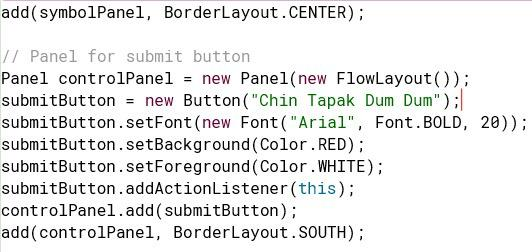
\includegraphics[width=0.8\textwidth]{code.jpeg} % Replace with actual image
    \caption{JAVA CODE}
\end{figure}

\noindent\textbf{Modifications:}
\begin{itemize}
    \item Font Size and Style: The font size and style have been adjusted for improved readability and consistency with the overall design.
    \item Background Color: The background color of the button has been updated to create a more visually appealing and cohesive look.
    \item Font Color: The font color has been modified to ensure strong contrast with the background, enhancing legibility.
    \item Element Proportions: Any disproportionate elements have been corrected to achieve a more balanced and aesthetically pleasing design.
\end{itemize}

\begin{figure}[h!]
    \centering
    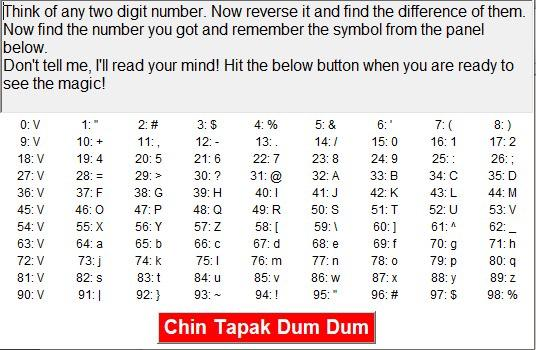
\includegraphics[width=0.8\textwidth]{output.jpeg} % Replace with actual image
    \caption{FINAL OUTPUT}
\end{figure}

\vspace{0.5cm}
\newpage

\section*{3. Calculator in C}
\textbf{Lab Entry by Arnab Pandit}

\subsection*{3.1 Introduction}
In this document, I will present a detailed explanation of a simple calculator program developed in the C programming language. This calculator performs various arithmetic operations including addition, subtraction, multiplication, division, percentage calculation, squaring, and cubing of numbers. The design of this calculator is aimed at providing a user-friendly interface with robust input validation to ensure accurate results.

\subsection*{3.2 Code}
Below is the complete code for the calculator in C, followed by an explanation of each function and its role in the program.

\begin{verbatim}
#include <stdio.h>
#include <math.h>
#include <stdlib.h>

// Function declarations
void addition();
void subtract();
void multiply();
void divide();
void percentage();
void square();
void cube();

int main() {
    int op;
    do {
        printf("Select an operation to perform in the C Calculator:\n");
        printf("1. Addition\n");
        printf("2. Subtraction\n");
        printf("3. Multiplication\n");
        printf("4. Division\n");
        printf("5. Percentage\n");
        printf("6. Square\n");
        printf("7. Cube\n");
        printf("8. Exit\n");
        printf("Please make a choice: ");
        
        // Validate user input
        while (scanf("%d", &op) != 1) {
            printf("Invalid input! Please enter a number between 1 and 8: ");
            while (getchar() != '\n'); // Clear the invalid input
        }
        
        // Perform the selected operation
        switch (op) {
            case 1: addition(); break;
            case 2: subtract(); break;
            case 3: multiply(); break;
            case 4: divide(); break;
            case 5: percentage(); break;
            case 6: square(); break;
            case 7: cube(); break;
            case 8: printf("Exiting the program.\n"); exit(0); // Exit the program
            default: printf("Error! Invalid choice. Try again.\n");
        }
        printf("\n*\n");
    } while (op != 8); // Repeat until the user chooses to exit
    return 0;
}
\end{verbatim}
% Continue with function definitions and explanations

\subsection*{3.3 Function Definitions}

\noindent \textbf{Addition Function:}
\begin{verbatim}
void addition() {
    int i, num;
    double sum = 0;
    printf("How many numbers do you want to add? ");
    
    // Read the number of inputs and validate it
    while (scanf("%d", &num) != 1 || num <= 0) {
        printf("Invalid input! Enter a positive number: ");
        while (getchar() != '\n'); // Clear the invalid input
    }
    
    printf("Enter the numbers:\n");
    for (i = 1; i <= num; i++) {
        double f_num;
        while (scanf("%lf", &f_num) != 1) {
            printf("Invalid input! Enter a valid number: ");
            while (getchar() != '\n'); // Clear the invalid input
        }
        sum += f_num;
    }
    
    // Display the result
    printf("Total sum of the numbers = %.2lf\n", sum);
}
\end{verbatim}

\noindent \textbf{Subtraction Function:}
\begin{verbatim}
void subtract() {
    double n1, n2;
    printf("Enter the first number: ");
    scanf("%lf", &n1);
    printf("Enter the second number: ");
    scanf("%lf", &n2);
    printf("The result of %.2lf - %.2lf is: %.2lf\n", n1, n2, n1 - n2);
}
\end{verbatim}

\noindent \textbf{Multiplication Function:}
\begin{verbatim}
void multiply() {
    double n1, n2;
    printf("Enter the first number: ");
    scanf("%lf", &n1);
    printf("Enter the second number: ");
    scanf("%lf", &n2);
    printf("The result of %.2lf * %.2lf is: %.2lf\n", n1, n2, n1 * n2);
}
\end{verbatim}

\noindent \textbf{Division Function:}
\begin{verbatim}
void divide() {
    double n1, n2;
    printf("Enter the first number: ");
    scanf("%lf", &n1);
    printf("Enter the second number: ");
    scanf("%lf", &n2);
    
    if (n2 != 0) {
        printf("The result of %.2lf / %.2lf is: %.2lf\n", n1, n2, n1 / n2);
    } else {
        printf("Error! Division by zero is not allowed.\n");
    }
}
\end{verbatim}

\newpage

\noindent \textbf{Percentage Function:}
\begin{verbatim}
void percentage() {
    double value, percent;
    printf("Enter the value: ");
    scanf("%lf", &value);
    printf("Enter the percentage: ");
    scanf("%lf", &percent);
    printf("%.2lf percent of %.2lf is: %.2lf\n", percent, value, (percent / 100) * value);
}
\end{verbatim}

\noindent \textbf{Square Function:}
\begin{verbatim}
void square() {
    double n1;
    printf("Enter a number to get the square: ");
    scanf("%lf", &n1);
    printf("The square of %.2lf is: %.2lf\n", n1, n1 * n1);
}
\end{verbatim}

\noindent \textbf{Cube Function:}
\begin{verbatim}
void cube() {
    double n1;
    printf("Enter a number to get the cube: ");
    scanf("%lf", &n1);
    printf("The cube of %.2lf is: %.2lf\n", n1, n1 * n1 * n1);
}
\end{verbatim}

\subsection*{3.4 Conclusion}
In conclusion, the simple calculator program developed in C provides a comprehensive tool for performing basic arithmetic operations. This calculator covers a range of functions including addition, subtraction, multiplication, division, percentage calculation, and the computation of squares and cubes of numbers. Each function is designed with user-friendly prompts and robust input validation to ensure accuracy and ease of use.

The program demonstrates effective use of functions to modulate the code, making it both organized and easy to maintain. By implementing input validation and error handling, the calculator minimizes the risk of user errors and enhances the overall user experience.

This project not only highlights fundamental programming concepts such as function definition and control structures but also showcases practical application in developing tools for everyday use. This simple calculator serves as a solid foundation for building more complex applications and improving programming skills in C.

\newpage
% Lab Entry 4: Pritam Pratihar
\section*{Lab Entry By Pritam Pratihar}
\subsection*{4. Creating LaTeX Repository on GitHub}

\subsubsection*{4.1 Introduction}
In this lab entry, we will walk through the steps to create a LaTeX repository on GitHub. GitHub is a popular platform for version control and collaboration, allowing users to store their LaTeX projects, track changes, and share them with others.

\subsubsection*{4.2 Steps for Creating the LaTeX Repository}

\textbf{Step 1: Creating a Repository on GitHub}
\begin{enumerate}
    \item Log in to your GitHub account at \url{https://github.com}.
    \item Click on the "New repository" button in the top right corner of your dashboard.
    \item Give your repository a name, for example, \texttt{my-latex-project}.
    \item Optionally, add a description for your repository.
    \item Choose whether you want the repository to be public or private.
    \item Click the \texttt{Create repository} button.
\end{enumerate}

\textbf{Step 2: Setting Up LaTeX Project Locally}
\begin{enumerate}
    \item Navigate to the folder where you want to store your project.
    \item Initialize a Git repository by running the command:
    \begin{verbatim}
    git init
    \end{verbatim}
    \item Create a LaTeX file, for example:
    \begin{verbatim}
    touch main.tex
    \end{verbatim}
\end{enumerate}

\textbf{Step 3: Connecting Your Local Repository to GitHub}
\begin{enumerate}
    \item Run the following command to link your local repository to GitHub:
    \begin{verbatim}
    git remote add origin https://github.com/your-username/my-latex-project.git
    \end{verbatim}
    \item Add and commit your changes:
    \begin{verbatim}
    git add .
    git commit -m "Initial commit"
    \end{verbatim}
    \item Push your changes to GitHub:
    \begin{verbatim}
    git push -u origin master
    \end{verbatim}
\end{enumerate}

\textbf{Step 4: Managing Your LaTeX Project on GitHub}
Once your repository is set up, you can continue working on your LaTeX project and commit changes as you make progress. GitHub allows for collaboration with others, so you can invite team members to contribute to your project.

\subsubsection*{4.3 Conclusion}
By hosting your LaTeX projects on GitHub, you benefit from version control and the ability to collaborate easily with others. The steps outlined above allow you to create and manage a LaTeX repository effectively.

\newpage
% Lab Entry 5: Suhana Pervaze
\section*{Lab Entry By Suhana Pervaze}
\subsection*{5. Introduction to LaTeX}

\subsubsection*{5.1 Introduction}
LaTeX is a typesetting system that is widely used for creating scientific and academic documents. It is especially well-suited for documents that contain complex mathematical equations, symbols, and citations. LaTeX provides a way to produce high-quality, professional documents that are consistent in layout and formatting.

\textbf{Key Features of LaTeX:}
\begin{itemize}
    \item \textbf{Mathematical Typesetting}: LaTeX excels in rendering mathematical symbols, equations, and structures like fractions, integrals, and matrices with precision.
    \item \textbf{Bibliographies and Citations}: LaTeX integrates with tools like BibTeX for managing references, making it easy to handle large bibliographies in academic papers.
    \item \textbf{Document Structuring}: LaTeX allows users to organize their documents into sections, subsections, and chapters, ensuring a clean and navigable structure.
    \item \textbf{Cross-referencing}: LaTeX offers robust features for referencing figures, tables, sections, and equations throughout the document.
    \item \textbf{Custom Formatting}: Users have extensive control over the appearance of the document, from font selection to spacing, margins, and headers/footers.
\end{itemize}

\subsubsection*{5.2 Basic LaTeX Commands}
Here are a few essential commands to get started with LaTeX: 

\textbf{Document Structure:}
\begin{verbatim}
\documentclass{article}
\begin{document}
\title{My First Document}
\author{Suhana Pervaze}
\date{\today}
\maketitle
\end{document}
\end{verbatim}

This code creates a simple LaTeX document with a title, author, and date. \\


\textbf{Sections and Subsections:}
\begin{verbatim}
\section{Introduction}
This is the introduction section.
\subsection{Background}
This is a subsection under the Introduction.
\end{verbatim}

\textbf{Mathematical Equations:}
\begin{verbatim}
The quadratic formula is given by:
\[
x = \frac{-b \pm \sqrt{b^2 - 4ac}}{2a}
\]
\end{verbatim}

\textbf{Inserting Images:}
\begin{verbatim}
\usepackage{graphicx}
\begin{figure}[h!]
    \centering
    \includegraphics[width=0.5\textwidth]{example-image}
    \caption{Example Image}
\end{figure}
\end{verbatim}

\subsubsection*{5.3 Conclusion}
LaTeX is a powerful tool for producing high-quality documents. Although it has a steep learning curve, its ability to handle complex formatting makes it indispensable for academic writing. Learning the basics of LaTeX can significantly enhance your document preparation process, particularly for technical and academic content.
\end{document}
